\documentclass{article}
\usepackage{fullpage,algorithmic,verbatim,graphicx,url,tikz,enumitem}
%\usepackage{ulem} %For strike-through text

\title{Evolutionary Computing\\
        COMP 5660-001/6660-001/6660-D01 -- Auburn University\\
        Fall 2021 -- Assignment Series 2\\
        GPac: A Genetic Programming \& Co-evolution Approach to the Game of Pac-Man}
\author{Deacon Seals\\
Braden Tisdale\\
Daniel Tauritz, Ph.D.}
\date{\today}

\begin{document}
\maketitle

\section*{Synopsis}
The goal of this assignment set is for you to become familiarized with (I) unambiguously formulating complex problems in terms of optimization, (II) implementing an Evolutionary Algorithm (EA) of the Genetic Programming (GP) persuasion, (III) conducting scientific experiments involving EAs, (IV) statistically analyzing experimental results from stochastic algorithms, and (V) writing proper technical reports. The problem you will be solving is to employ GP to first evolve a controller for Pac-Man (also referred to as a Pac-Man agent) and subsequently to co-evolve controllers for Pac-Man with maps. This problem is representative of a large and very important class of problems which require the identification of system models such as controllers, programs, or equations. An example of the latter is symbolic regression which attempts to identify a system model based on a limited number of observations of the system's behavior; classic mathematical techniques for symbolic regression have certain inherent limitations which GP can overcome. Employing GP to evolve a controller for Pac-Man is also a perfect illustration of how GP works, while avoiding many of the complications of evolving full blown computer programs.

These are individual assignments and plagiarism will not be tolerated. You must write your code from scratch in one of the approved programming languages. You are free to use libraries/toolboxes/etc, except problem and search/optimization/EA specific ones.

\section*{Problem statement}
In this assignment you will implement and evolve controllers for Pac-Man and co-evolve against maps.

\subsection*{GPac}
In GPac, the world is a two-dimensional grid and there is no world wrap. There are two types of units: Pac-Man and the Ghosts. Pac-Man always starts at the top left cell and all three the ghosts always start at the bottom right cell. These units are guided by controllers, which is what your GP will evolve. Units move in cardinal directions (up, down, left, right); Pac-Man can choose to hold position, but the Ghosts cannot. They move from one grid cell to another in a discrete fashion (i.e., they move a whole cell at a time). Units cannot move off the edges of the map. Ghosts can occupy the same grid cell as other ghosts. If Pac-Man and a Ghost occupy the same cell, the game is over. If Pac-Man and a Ghost collide (i.e., exchange cells), the game is over.

% \subsubsection*{Walls}
% To relieve you from the burden of creating Pac-Man maps -- which is both a science and an art! -- you are provided 100 guaranteed solvable maps that you need to uniform randomly sample from. Note that nothing can be placed in, or move through, a cell with a wall. The format of the map files is as follows: the first line contains two integers, the first being the width and the second the height, both with a minimum value of two; the following lines consist of octothorpes (\#) and tildes ($\sim$) where \# indicates that a cell contains wall and a $\sim$ indicates that a cell does not contain wall. 

\subsubsection*{Pills}
Before the game begins, cells are chosen at random according to a preset pill-density parameter to contain ``pills''. The pill-density parameter specifies the percentage chance for any given cell to contain a pill, subject to the constraints (a) at least one cell needs to contain a pill, (b) pills cannot be placed in walls and (c) Pac-Man's starting cell cannot contain a pill. Thus: \emph{E[number of cells containing a pill] = MAX (1 , pill-density $\cdot$ (total number of cells - 1 - number of walls))}

If Pac-Man occupies a cell that contains a pill, the pill is removed, and Pac-Man's score is increased. When all pills have been removed from the world, the game is over. 

\subsubsection*{Fruit}
Each turn that the game is running, there is a user-configurable chance for a piece of fruit to spawn. There can only be one piece of fruit on the field at a time and it may not spawn in the same cell as a pill, a wall, or Pac-Man's current cell. If Pac-Man occupies the cell that contains the piece of fruit, the fruit is removed, and Pac-Man's score is increased by the fruit score which is user-configurable.

\subsubsection*{Time}
Each GPac game starts with time equal to the number of grid cells in the world multiplied by the time multiplier. Each turn is one time step.  When the time limit reaches zero, the game is over. This prevents games from getting stuck in infinite loops. It also promotes efficient controller evolution.

\subsubsection*{Game Play}
Each turn, the game gives each of the unit's controllers the current game state. This state includes at least: where all of the units are currently located and where all of the pills are located. Each controller will then choose what move to make (up, down, left, right for all controllers, also hold just for Pac-Man). Once all of the units have determined their next move, the game state will update everyone's position and decrease the time remaining by one. Once everyone has moved, the game will check if:
\begin{enumerate}
\item Pac-Man and any of the Ghosts are in the same cell, causing game-over.
\item Pac-Man collided with a Ghost, causing game-over.
\item Pac-Man is in a cell with a pill, causing the pill to be removed, and the score to be adjusted.
\item Pac-Man is in a cell with a piece of fruit, causing the fruit to be removed, and the score to be adjusted.
\item All the pills are removed, causing game-over.
\item Time remaining is equal to zero, causing game-over.
\end{enumerate}

\subsubsection*{Score}
Pac-Man's score is equal to the percentage of the total number of pills he has consumed truncated to an integer, \emph{plus} the score for fruit consumed. If the game ends because there are no more pills on the board, Pac-Man's score is increased by the percentage of time remaining truncated to an integer. This score can be used directly for the fitness of the Pac-Man controller. Ghost fitness should be inversely proportional to Pac-Man's fitness (for example, negate his fitness) and if the game ends due to Pac-Man's demise, then the Ghost score is increased by the percentage of time remaining truncated to an integer.

\section*{World File Format}
GPac generates a sequence of your world states for a single run to facilitate debugging, visualization, and grading. The common file format you are required to use consists of header values for the width and height of the world, followed by, for each snap shot that you are outputting, a list of ordered triples consisting of $<$key$><$space$><$value$><$space$><$value$>$. The origin (0,0) is in the lower-left corner. The valid triples are:
\begin{itemize}
\item[m] Pac-Man; second value is x-coordinate; third value is y-coordinate
\item[1] Ghost 1; second value is x-coordinate; third value is y-coordinate
\item[2] Ghost 2; second value is x-coordinate; third value is y-coordinate
\item[3] Ghost 3; second value is x-coordinate; third value is y-coordinate
\item[p] Pill; second value is x-coordinate; third value is y-coordinate
\item[w] Wall; second value is x-coordinate; third value is y-coordinate
\item[f] Fruit spawned; second value is x-coordinate; third value is y-coordinate
\item[t] End of current turn; second value is remaining time; third value is current score
\end{itemize}
Note that you only need to write out the pill and wall locations during the first snap shot as the moves of Pac-Man implicitly define the pill locations of all later snap shots. This will make your world file significantly smaller in size.
\noindent Here is an example file for a world with width 40, height 30, 3 snap shots, and 3 pills:
\begin{verbatim}
40
30
m 0 29
1 39 0
2 39 0
3 39 0
w 1 1
w 36 20
w 10 10
w 2 29
p 1 29
p 36 19
p 27 8
t 2400 0
m 1 29
1 38 0
2 38 0
3 39 1
t 2399 33
m 1 28
1 38 1
2 37 0
3 39 0
t 2398 33
\end{verbatim}

\section*{General implementation requirements}
For this assignment series you must implement GPac controllers for Pac-Man. You are provided with an implementation of GPac with proper score calculation, spawn mechanics, game-over identification, and world file generation (called a game log in the code). In theory, the fitness of a controller is its expected performance for an arbitrary game instance (i.e., its performance averaged over all game instances). However, as it is computationally infeasible to evaluate a controller over all possible game instances, for the purpose of this assignment it will be sufficient to play a single game instance to completion to estimate fitness. Your code needs to be compatible with the provided GPac implementation and adhere to the specifications of the individual assignments in this series. Your submission should also compile and execute within the base Conda Linux environment as prescribed in the environment setup assignment. If you require a package not present in that base environment, please contact a TA for approval. In all assignments that contain Jupyter notebooks: those notebooks must be completed and submitted with results from running the full notebook.

The GP controllers must be implemented as follows: for each valid action and the corresponding new state from executing the action, apply the state evaluator encoded in the GP tree, returning the valid action with the best state evaluation. The terminal nodes consist of sensor inputs and floating point constants. The function nodes consists of mathematical operators which take as input floating point numbers and provide as output floating point numbers as well. You need to implement at minimum four sensor inputs, where the target location specifically refers to the grid cell where the controller's unit is moving to this turn, namely: (1) the Manhattan distance between the target location and the nearest Ghost, (2) the Manhattan distance between the target location and the nearest pill, (3) the number of walls immediately adjacent to the target location, and (4) the Manhattan distance between the target location and the fruit. Note: When considering a move in which a pill or the fruit is consumed, immediately increasing the Pac-Man to pill or fruit distance input may lead your controllers to think that the new state is worse than the state prior to eating the fruit. You need to implement at minimum five mathematical operators, namely: (1) addition, (2) subtraction, (3) multiplication, (4) division, and (5) rand($a$,$b$) which returns uniform randomly a number between $a$ and $b$.

The highest-score-game-sequence all-time-step world file is a file in the previously specified World File Format containing a sequence of world states at every time step of typically the best run of your experiment (i.e., the run with the global best fitness). In 2a \& 2b the solution file should contain the best Pac-Man controller found, in 2c the solution files should contain the best Pac-Man controller and map found respectively. 

The solution file format must be exactly as follows to allow automated format checking: you need to output your parse tree(s) such that each tree node is on a new line in the format \textless `\textbar` characters corresponding to tree depth\textgreater\textless node character\textgreater, where the root of the tree is at depth 0 and the following characters represent tree nodes:
\begin{itemize}
\item Sensor inputs
    \begin{description}
    \item[G] Manhattan distance to nearest ghost 
    \item[P] Manhattan distance to nearest pill 
    \item[W] Number of immediately adjacent walls 
    \item[F] Manhattan distance to nearest fruit 
    \item[\#.\#] Constant value (where the `\#` character is replaced with a one or more digits) 
    \end{description}
\item Operators
    \begin{description}
    \item[+] Addition 
    \item[-] Subtraction 
    \item[*] Multiplication 
    \item[/] Division 
    \item[RAND] Random number between two children node values. 
    \end{description}
\end{itemize}
All of the above operators should have strictly two children.  

For the sensor inputs P and F, if a move would place Pac-Man on top of a pill or fruit, the sensor value should be 0, rather than considering the item as collected and gone. If there is no fruit, then F should have a constant value.

Note: you are encouraged to implement additional sensor inputs and operators with your own (well documented) single or multiple character representations. These new operators are not bound to the strict two children constraint of the required operators, but make sure you document the degree or range of acceptable degrees for your operators. Additional sensor nodes often lead to interesting agent capabilities and strategies. 
 
\subsection*{Example}
Here is an example parse tree:\\

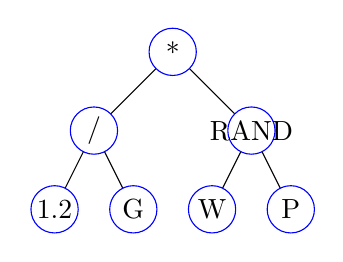
\begin{tikzpicture}
\draw (3,2) -- (2,1); \draw (3,2) -- (4,1);
\draw [blue] [fill=white] (3,2) circle [radius=0.3]; \node at (3,2) {*}; 
\draw (2,1) -- (1.5,0); \draw (2,1) -- (2.5,0); \draw (4,1) -- (3.5,0); \draw (4,1) -- (4.5,0);
\draw [blue] [fill=white] (2,1) circle [radius=0.3]; \node at (2,1) {/};
\draw [blue] [fill=white] (4,1) circle [radius=0.3]; \node at (4,1) {RAND};
\draw [blue] [fill=white] (1.5,0) circle [radius=0.3]; \node at (1.5,0) {1.2};
\draw [blue] [fill=white] (2.5,0) circle [radius=0.3]; \node at (2.5,0) {G};
\draw [blue] [fill=white] (3.5,0) circle [radius=0.3]; \node at (3.5,0) {W};
\draw [blue] [fill=white] (4.5,0) circle [radius=0.3]; \node at (4.5,0) {P};
\end{tikzpicture}\\

\noindent The parse tree shown above would look as follows in a solution file: 
\begin{verbatim}
* 
|/ 
||1.2 
||G 
|RAND 
||W 
||P 
\end{verbatim}



\section*{Version control requirements}
For each assignment you will be given a new repository on [\url{https://classroom.github.com}]. \textbf{Please view your repository and the README.md file}. It may clear things up after reading this.

Included in your repository is a script named ``finalize.sh'', which you will use to indicate which version of your code is the one to be graded. When you are ready to submit your final version, run the command \texttt{./finalize.sh} from your local Git directory, then commit and push your code. This will create a text file, ``readyToSubmit.txt'', that is pre-populated with a known text message for grading purposes. You may commit and push as much as you want, but your submission will be confirmed as ``final'' if  ``readyToSubmit.txt'' exists and is populated with the text generated by ``finalize.sh'' at 10:00pm on the due date. If you do not plan to submit before the deadline, then you should NOT run the ``finalize.sh'' script until your final submission is ready. If you accidentally run ``finalize.sh'' before you are ready to submit, do not commit or push your repo and delete ``readyToSubmit.txt''. Once your final submission is ready, run ``finalize.sh'', commit and push your code, and do not make any further changes to it.

The code currently pushed to the default branch will be pulled for grading. The TAs should not have to worry about external dependencies. Any files created by your assignment must be created in the present working directory or its subfolders.


\section*{Submissions, penalties, documents, and bonuses}
You may commit and push to your repository at anytime. At submission time, your latest, pushed and finalized, commit to the master branch will be graded (if there is one). In order to ensure that the correct version of your code will be used for grading, after pushing your code, visit [\url{https://github.com}] and verify that your files are present. If for any reason you submit late, then \textbf{please notify the TAs when you have submitted.} If you do submit late, then your first late submission will be graded.

The penalty for late submission is a 5\% deduction for the first 24 hour period and a 10\% deduction for every additional 24 hour period. So 1 hour late and 23 hours late both result in a 5\% deduction. 25 hours late results in a 15\% deduction, etc. Not following submission guidelines can be penalized for up to 5\%, which may be in addition to regular deduction due to not following the assignment guidelines.

Your code needs to compile/execute as submitted without syntax errors and without runtime errors. Grading will be based on what can be verified to work correctly as well as on the quality of your source code. You must follow the coding requirements as stated in the syllabus.

Documents are required to be in PDF format; you are encouraged to employ \LaTeX~for typesetting.

Note that the first two assignments in this series are weighted equally, but the third and last counts double to allow you one extra chance to significantly makeup your assignment grade.


\section*{Deliverable Categories}
There are three deliverable categories, namely:
\begin{description}
\item[GREEN] Required for all students in all sections.
\item[YELLOW] Required for students in the 6000-level sections, bonus for the students in the 5000-level section.
\item[RED] Bonus for all students in all sections.
\end{description}
Note that the max grade for the average of all assignments in Assignment Series 2, including bonus points, is capped at 100\%.

\newpage

%-------------------------------------------------------------------------------------------------------------------------------------------------------------------------------------------------
\section*{Assignment 2a: Random Search}
You must implement a random search through valid parse tree space for Pac-Man controllers in GPac. In this assignment, you are asked to complete the Jupyter notebook \texttt{2a\_notebook.ipynb} and several other Python files as directed by the notebook. Your submission should also contain a report to document the findings of a 30-run experiment as well as files containing the world file (log) and tree from the solution with the highest fitness from all runs. In your report, include a stair-step plot showing the progression of number of fitness evaluations versus local best fitness for the run that produced the highest fitness overall, the standard deviation and mean of the best fitness found from each run, and an informal analysis of your agent's performance from watching the visualization of the highest-fitness solution. In this informal analysis, we want you to comment on whether or not you think the agent performs well, as well as any notable behavioral quirks.

The deliverables of this assignment are:
\begin{description}
\item[GREEN 1] your source code and completed notebook
\item[GREEN 2] a PDF document headed by your name, AU E-mail address, and the string ``COMP x66y Fall 2021 Assignment 2a'', where $x$ and $y$ need to reflect the section you are enrolled in, containing your report, including statistical analysis and plot(s)
\item[GREEN 3] files containing any data you analyzed to write your report or generate your plot(s), in a format that can be easily understood by the TAs (if you think you might should include instructions on how to interpret your data, then you should!), as well as the highest-score-game-sequence all-time-step world files, and solution files (these should go in the repo's \emph{worldFiles}, and \emph{solutions} directories respectively).
\item[RED 1] In order to demonstrate that an EA is a reasonable tool for solving a given problem, it is generally more compelling to compare the EA to a simple optimization algorithm such as a hill climber, rather than random search. Showing that the EA outperforms a hill climber indicates that the problem being solved is probably multimodal, and that evolution allows a more effective exploration of the search space. Up to 15\% bonus points can be earned by investigating the use of a hill climber to optimize controllers by making small changes to the controller and accepting changes that improve fitness. This bonus investigation needs to be documented, including result plots and a new config file, in a separate section of the required document marked as ``Hill Climber''. You also need to indicate in your source files any code which pertains to this bonus and additionally describe it in your README.md file. Basically, you need to make it as easy as possible for the TAs to see with a glance what part of your submission pertains to this bonus, and which does not.
\end{description}
Edit your README.md file to explain anything you feel necessary. Submit all files via GitHub, by \emph{pushing} your latest commit to the \emph{master} branch. The due date for this assignment is 10:00 PM on Sunday October 24, 2021.
\\
\\
\textbf{Grading}\\
The point distribution is as follows:\\
\\
\begin{tabular}{l|l|l}
    Assessment Rubric $\backslash$ Deliverable Category & Green & Red\\ \hline \hline
	Algorithmic comprehension                                       & 50 & 55 \\
	\hline Logging and output files            & 15 & 5 \\
	\hline Good programming including code reliability, commenting, correctness, \& practices & 10 & 10\\
	\hline Report        & 25 & 30 \\
\end{tabular}\\

\newpage

\section*{Assignment 2b: Genetic Programming Search}
You need to evolve a GP tree controller for Pac-Man which generates the most high-quality valid action out of the 5 possible actions for Pac-Man that it can find, employing the approach described in the general specification. The map should be the same static map as specified in Assignment~2a. In this assignment, you are asked to complete the Jupyter notebook \texttt{2b\_notebook.ipynb} and several other Python files as directed by the notebook.

You need at minimum to implement support for the following EA configurations, as described in the notebook:
\begin{description}
\item[Representation] Tree
\item[Initialization] Ramped half-and-half (see Section 6.4 in \cite{Eiben2015})
\item[Parent Selection] Fitness Proportional Selection, $k$-Tournament Selection without replacement, uniform random selection
\item[Recombination] Sub-Tree Crossover
\item[Mutation] Sub-Tree Mutation
\item[Survival Selection] Truncation, $k$-Tournament Selection without replacement
\item[Bloat Control] Parsimony Pressure
\item[Termination] Number of fitness evaluations
\end{description}

Your submission should also contain a report to document the findings of a 30-run experiment as well as files containing the world file (log) and tree from the solution with the highest fitness from all runs. In your report, include the following:
\begin{itemize}
    \item a plot showing fitness evaluations versus best and average population fitness averaged over 30 runs (like Assignments 1b-1d)
    \item statistical analysis (F-test and t-test) comparing the best fitness obtained by each run to the data generated by the search algorithm in Assignment 2a
    \item a brief discussion interpreting the results of the statistical tests
    \item an informal comparison of the behavior of the best Assignment 2a agent and the best GP agent from watching the visualization of the highest-scoring solutions from each algorithm
\end{itemize}

The deliverables of this assignment are:
\begin{description}
\item[GREEN 1] your source code and completed notebook
\item[GREEN 2] a PDF document headed by your name, AU E-mail address, and the string ``COMP x66y Fall 2021 Assignment 2b'', where $x$ and $y$ need to reflect the section you are enrolled in, containing your report, including statistical analysis and plot(s)
\item[GREEN 3] files containing any data you analyzed to write your report or generate your plot(s), in a format that can be easily understood by the TAs (if you think you might should include instructions on how to interpret your data, then you should!), as well as the highest-score-game-sequence all-time-step world files, and solution files (these should go in the repo's \emph{worldFiles}, and \emph{solutions} directories respectively).

\item[YELLOW 1] Investigate the role of parsimony pressure with respect to both parsimony technique (e.g., tree depth versus tree size) and parsimony coefficient (i.e., the amount of penalty incurred for bloat). This bonus investigation needs to be documented, including fitness evaluations versus a relevant tree complexity metric as well as the usual fitness evaluations versus best and average fitness plots averaged over all runs, and also including appropriate statistical analysis, in a separate section of your report marked as ``Parsimony Investigation''. You also need to indicate in your source files any code which pertains to this bonus and additionally describe it in your report. Basically, you need to make it as easy as possible for the TAs to see with a glance what part of your submission pertains to this deliverable.
Students enrolled in COMP 5660 can earn up to 15\% bonus for this investigation. For students enrolled in COMP 6660 this will count for 15\% regular points (not bonus) beyond the GREEN deliverables. 

\item[RED 1] Up to 10\% bonus points can be earned by investigating having multiple simultaneous Pac-Man's all employing \emph{identical} controllers, where they all have to die for the game to end, and they share the same score (i.e., there's no competition between the Pac-Man's). You should add appropriate additional terminals, such as ``Distance to nearest other Pac-Man''. This bonus investigation needs to be documented, including result plots, in a separate section of the required document marked as ``Multiple Identical Pac-Man Controllers''. Basically, you need to make it as easy as possible for the TAs to see with a glance what part of your submission pertains to this bonus, and which does not. See the notebook for details on modifying the \emph{play\_GPac} function to support this.
\item[RED 2] Up to 15\% bonus points can be earned by investigating the evolution of a controller that controls all ghosts, with the fitness of negative game score, and plays against a static Pac-Man strategy. You should add appropriate additional terminals, such as ``Distance to nearest Pac-Man'' and ``Distance to nearest other ghost''. This bonus investigation needs to be documented in a separate section of the required document marked as ``Multiple Identical Ghost Controllers''. You also need to indicate in your source files any code which pertains to this bonus and additionally describe it in your report. Basically, you need to make it as easy as possible for the TAs to see with a glance what part of your submission pertains to this bonus, and which does not. See the notebook for details on modifying the \emph{play\_GPac} function to support this. Performing competitive co-evolution with ghosts will be a bonus on Assignment 2c.

\end{description}
Include a readme file to explain anything you feel necessary. The due date for this assignment is 10:00 PM on Sunday November 7, 2021.
\\
\\
\textbf{Grading}\\
The point distribution per deliverable category is as follows: \\
\\
\begin{tabular}{l|l|l|l|}
  Assessment Rubric $\backslash$ Deliverable Category & Green       & Yellow        & Red\\ \hline \hline  
  Algorithmic                                                              & 50\% & 55\% & 65\%\\
  \hline Logging and output files                      & 10\%  & 5\%   & 5\%\\
  \hline Good programming including code reliability, commenting, correctness, \& practices      & 10\%  & 10\% & 10\%\\
  \hline Report    & 15\%  & 15\% & 20\% \\
  \hline Statistical analysis                                          &  15\%   & 15\% &0\%\\
\end{tabular}\\
\\
\newpage

\section*{Assignment 2c: Competitive Co-evolutionary Search}
You need to co-evolve within a configurable number of fitness evaluations, where a fitness evaluation is defined to be a single game played, a GP controller for Pac-Man which generates the supposedly optimal valid action out of the 5 possible actions for Pac-Man and a map that provides the supposedly optimal challenge for Pac-Man. The type of co-evolution you will be using is competitive co-evolution~\cite[Section 15.3]{Eiben2015} employing two populations, one for the Pac-Man controllers and one for the maps. The recommended GP and EA approaches are the same as in Assignment 2b and Assignment 1b for Pac-Man controllers and maps, respectively. In this assignment, you are asked to complete the Jupyter notebook \texttt{2c\_notebook.ipynb} and several other Python files as directed by the notebook.

You need at minimum to implement support for the following EA configurations, where operators with multiple options are comma separated, and operators need to be able to be configured independently for Pac-Man and maps respectively:
\begin{description}
\item[Pac-Man Representation] Tree
\item[Pac-Man Initialization] Ramped half-and-half (see Section 6.4 in \cite{Eiben2015})
\item[Pac-Man Parent Selection] Fitness Proportional Selection, $k$-Tournament Selection without replacement, uniform random selection
\item[Pac-Man Recombination] Sub-Tree Crossover
\item[Pac-Man Mutation] Sub-Tree Mutation
\item[Pac-Man Survival Selection] Truncation, $k$-Tournament Selection without replacement
\item[Pac-Man Bloat Control] Parsimony Pressure
\item[Map Representation] Fixed-length binary string
\item[Map Initialization] Uniform random binary strings
\item[Map Parent Selection] Fitness Proportional Selection, $k$-Tournament Selection without replacement, uniform random selection
\item[Map Recombination] Uniform, 1-Point
\item[Map Mutation] Binary String Mutation
\item[Map Survival Selection] Truncation, $k$-Tournament Selection without replacement
\item[Termination] Number of fitness evaluations
\end{description}

Note: If $\mu$ of the Pac-Man population is not equal to $\mu$  of the map population or $\lambda$ of the Pac-Man population is not equal to $\lambda$ of the map population, some controllers or maps will have to be used more than once to complete all fitness evaluations. If you use a controller or map more than once, simply take the average of all games the controller or map played for fitness and store the game log of the game that was better for the individual in question (e.g., Pac-Man uses the log with the higher score and a map uses the log with the lower score).\\


For each experiment in this assignment you are asked to submit highest-score-game-sequence all-time-step world files from an exhibition game (i.e., an extra match does not count as an evaluation) played between your best Pac-Man controller and Map from the final generation of the same run. Similarly, you will produce two solution files per experiment: one for the Pac-Man controller and one for the map used in this game. Note that for all deliverables except RED 4, acceptable statistical analysis consists of reporting the mean and standard deviation of the best fitness of the final generation of each species across all runs in your experiment.

The deliverables of this assignment are:
\begin{description}
\item[GREEN 1] your source code and completed notebook
\item[GREEN 2]  a document in PDF format headed by your name, AU E-mail address, and the string ``COMP x66y Fall 2021 Assignment 2c'', where $x$ and $y$ need to reflect the section you are enrolled in', containing:
  \begin{description}
  \item[Methodology] Describe the custom parts of your EA design, such as your function and terminal sets, as well as your approach to performing adversarial evaluations, in sufficient detail to allow someone else to implement a functionally equivalent EA, and explain your EA design decisions.
  \item[Experimental Setup] Provide your experimental setup in sufficient detail to allow exact duplication of your experiments (i.e., producing the exact same results within statistical margins) and justify your choice of EA strategy parameters.
  \item[Results] List your experimental results in both tabular (mean and standard deviation) and graphical formats (box plots preferred).
  \item[Discussion] Discuss any notable behavioral characteristics of the Pac-Man controllers when compared to the controllers found in Assignment 2b. In particular, we want you to report on how and if agent behavior changed in the presence of co-evolving maps.
  \item[Conclusion] Conclude your report by stating your most important findings and insights in the conclusion section. 
  \item[Bibliography] This is where you provide your citation details, if you cited anything. Only list references here that you actually cite in your report.
  \item[Appendices] If you have more data you want to show than what you could reasonably fit in the body of your report, this is the place to put it along with a short description.
  \end{description}
\item[GREEN 3] files containing any data you analyzed to write your report or generate your plot(s), in a format that can be easily understood by the TAs (if you think you might should include instructions on how to interpret your data, then you should!), as well as the highest-score-game-sequence all-time-step world files, and solution files (these should go in the repo's \emph{worldFiles}, and \emph{solutions} directories respectively).
\item[YELLOW 1] Investigate under what circumstances co-evolutionary cycling occurs in Pac-Man and maps and adding a section to the document to describe all aspects of your investigation, including CIAO plots~\cite{Cliff1995} to visualize your findings. You need to include all your related configuration, data, world, and solution files and clearly indicate in your source files any code which pertains to this deliverable. Basically, you need to make it as easy as possible for the TAs to see with a glance what part of your submission pertains to this deliverable, and which does not.
Students enrolled in COMP 5660 can earn up to 10\% bonus for this investigation. For students enrolled in COMP 6660 this will count for 10\% regular points (not bonus) beyond the GREEN deliverables. 

\item[RED 1] Up to 10\% bonus points can be earned by investigating the co-evolution of a controller that controls all ghosts, with the fitness of negative game score, and plays against co-evolving Pac-Man controllers on a static map. You should add appropriate additional terminals, such as ``Distance to nearest Pac-Man'' and ``Distance to nearest other ghost''. This bonus investigation needs to be documented in a separate section of the required document marked as ``Pac-Man and Ghost Co-Evolution''. You also need to indicate in your source files any code which pertains to this bonus and additionally describe it in your report. Basically, you need to make it as easy as possible for the TAs to see with a glance what part of your submission pertains to this bonus, and which does not.

\item[RED 2] Up to 10\% bonus points can be earned by investigating the cooperative co-evolution of a Ghost controller with a map using a static Pac-Man strategy and negative game score as fitness for both species. This bonus investigation needs to be documented in a separate section of the required document marked as ``Map and Ghost Cooperative Co-Evolution''. You also need to indicate in your source files any code which pertains to this bonus and additionally describe it in your report. Basically, you need to make it as easy as possible for the TAs to see with a glance what part of your submission pertains to this bonus, and which does not.

\item[RED 3] Up to 10\% bonus points can be earned by investigating 3-species co-evolution Pac-Man controllers, maps, and Ghost controllers. This bonus investigation needs to be documented in a separate section of the required document marked as ``3-Species Co-Evolution''. You also need to indicate in your source files any code which pertains to this bonus and additionally describe it in your report. Basically, you need to make it as easy as possible for the TAs to see with a glance what part of your submission pertains to this bonus, and which does not.

\item[RED 4] You may have noticed that this assignment doesn't contain any request for rigorous statistical analysis. This is because performing meaningful statistical analysis is often nuanced (and computationally expensive) for problems without an inherent absolute fitness metric (like GPac). For up to 10\% bonus points, design and implement a method for performing a meaningful, fair, and consistent comparison between solutions from any two co-evolution configurations/experiments co-evolving the same species, then perform statistical analysis using metrics obtained from your comparison method. Your method and statistical analysis results (with your interpretation of results) should be documented in a separate section of the required document marked as ``Statistical Analysis of Co-Evolution''. You also need to indicate in your source files any code which pertains to this bonus and additionally describe it in your report. Basically, you need to make it as easy as possible for the TAs to see with a glance what part of your submission pertains to this bonus, and which does not.

\end{description}
The due date for this assignment is 10:00 PM on Sunday November 28, 2021.
\\
\\
\textbf{Grading}\\
The point distribution per deliverable category is as follows (note that 2c has twice the points as 2a \& 2b): \\
\\
\begin{tabular}{p{20em}|l|l|l|l|}
  Assessment Rubric $\backslash$ Deliverable Category & Green       & Yellow        & Red 1-3 & Red 4\\ \hline \hline  
  Algorithmic                                                             & 45\% & 35\% & 40\% & 25\%\\
  \hline Logging and output/solution files                      & 10\% &  5\%  & 5\% & 5\%\\
  \hline Good programming including code reliability, commenting, correctness, \& practices       & 10\% & 10\% & 10\% & 10\%\\
  \hline Document                                                      & 25\%  & 40\% & 35\% & 30\%\\
  \hline Statistical analysis                                           & 10\%  & 10\% & 10\% & 30\%\\
\end{tabular}

\begin{thebibliography}{10}

\bibitem{Eiben2015}
A.~E.~Eiben and J.~E.~Smith, \textit{Introduction to Evolutionary Computing}. Second Edition, Springer-Verlag, Berlin Heidelberg, 2015, ISBN 978-3-662-44873-1.

\bibitem{Cliff1995}
Dave Cliff and Geoffrey F. Miller, \textit{Tracking the red Queen: Measurements of Adaptive Progress in Co-Evolutionary Simulations}. In Advances in Artificial Life, Lecture Notes in Computer Science, Volume 929, Pages 200-218, Springer-Verlag, Berlin Heidelberg, 1995, ISBN 978-3-540-59496-3. \url{http://www.cs.uu.nl/docs/vakken/ias/stuff/cm95.pdf}

\end{thebibliography}

\end{document}